% Created by tikzDevice version 0.12.6 on 2024-03-19 17:31:37
% !TEX encoding = UTF-8 Unicode
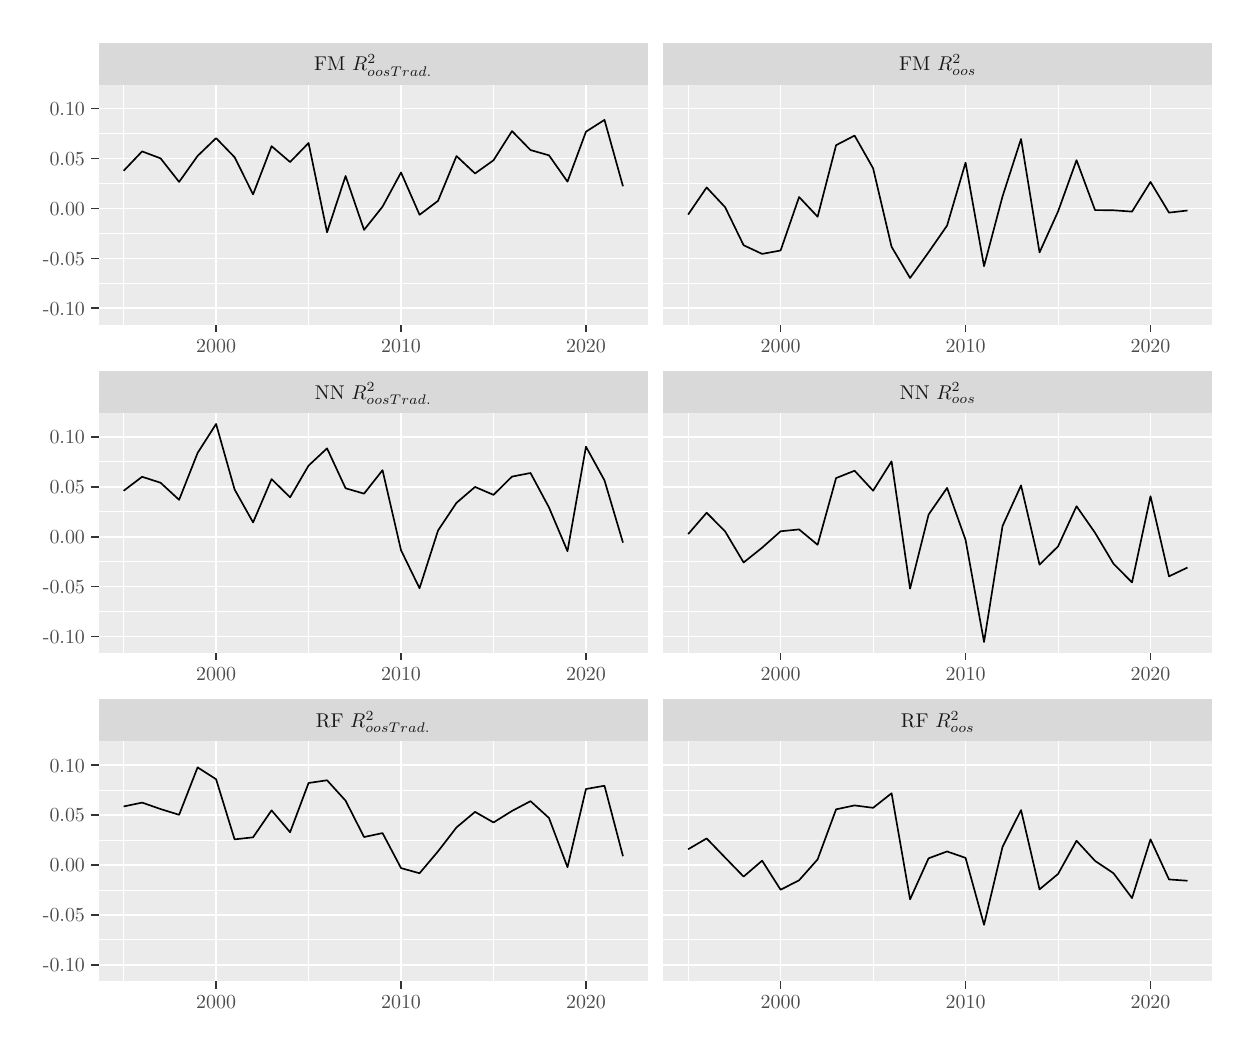
\begin{tikzpicture}[x=1pt,y=1pt]
\definecolor{fillColor}{RGB}{255,255,255}
\path[use as bounding box,fill=fillColor,fill opacity=0.00] (0,0) rectangle (433.62,361.35);
\begin{scope}
\path[clip] (  0.00,  0.00) rectangle (433.62,361.35);
\definecolor{drawColor}{RGB}{255,255,255}
\definecolor{fillColor}{RGB}{255,255,255}

\path[draw=drawColor,line width= 0.6pt,line join=round,line cap=round,fill=fillColor] (  0.00,  0.00) rectangle (433.62,361.35);
\end{scope}
\begin{scope}
\path[clip] ( 25.65,254.04) rectangle (224.13,340.69);
\definecolor{fillColor}{gray}{0.92}

\path[fill=fillColor] ( 25.65,254.04) rectangle (224.13,340.69);
\definecolor{drawColor}{RGB}{255,255,255}

\path[draw=drawColor,line width= 0.3pt,line join=round] ( 25.65,268.97) --
	(224.13,268.97);

\path[draw=drawColor,line width= 0.3pt,line join=round] ( 25.65,287.00) --
	(224.13,287.00);

\path[draw=drawColor,line width= 0.3pt,line join=round] ( 25.65,305.03) --
	(224.13,305.03);

\path[draw=drawColor,line width= 0.3pt,line join=round] ( 25.65,323.07) --
	(224.13,323.07);

\path[draw=drawColor,line width= 0.3pt,line join=round] ( 34.67,254.04) --
	( 34.67,340.69);

\path[draw=drawColor,line width= 0.3pt,line join=round] (101.50,254.04) --
	(101.50,340.69);

\path[draw=drawColor,line width= 0.3pt,line join=round] (168.33,254.04) --
	(168.33,340.69);

\path[draw=drawColor,line width= 0.6pt,line join=round] ( 25.65,259.95) --
	(224.13,259.95);

\path[draw=drawColor,line width= 0.6pt,line join=round] ( 25.65,277.98) --
	(224.13,277.98);

\path[draw=drawColor,line width= 0.6pt,line join=round] ( 25.65,296.02) --
	(224.13,296.02);

\path[draw=drawColor,line width= 0.6pt,line join=round] ( 25.65,314.05) --
	(224.13,314.05);

\path[draw=drawColor,line width= 0.6pt,line join=round] ( 25.65,332.08) --
	(224.13,332.08);

\path[draw=drawColor,line width= 0.6pt,line join=round] ( 68.08,254.04) --
	( 68.08,340.69);

\path[draw=drawColor,line width= 0.6pt,line join=round] (134.91,254.04) --
	(134.91,340.69);

\path[draw=drawColor,line width= 0.6pt,line join=round] (201.74,254.04) --
	(201.74,340.69);
\definecolor{drawColor}{RGB}{0,0,0}

\path[draw=drawColor,line width= 0.6pt,line join=round] ( 34.67,309.62) --
	( 41.35,316.64) --
	( 48.03,314.12) --
	( 54.72,305.61) --
	( 61.40,315.00) --
	( 68.08,321.44) --
	( 74.77,314.53) --
	( 81.45,301.12) --
	( 88.13,318.52) --
	( 94.82,312.80) --
	(101.50,319.67) --
	(108.18,287.42) --
	(114.87,307.76) --
	(121.55,288.27) --
	(128.23,296.67) --
	(134.91,309.02) --
	(141.60,293.74) --
	(148.28,298.76) --
	(154.96,314.96) --
	(161.65,308.66) --
	(168.33,313.43) --
	(175.01,323.97) --
	(181.70,317.13) --
	(188.38,315.21) --
	(195.06,305.70) --
	(201.74,323.76) --
	(208.43,328.02) --
	(215.11,304.04);
\end{scope}
\begin{scope}
\path[clip] ( 25.65,135.43) rectangle (224.13,222.07);
\definecolor{fillColor}{gray}{0.92}

\path[fill=fillColor] ( 25.65,135.43) rectangle (224.13,222.07);
\definecolor{drawColor}{RGB}{255,255,255}

\path[draw=drawColor,line width= 0.3pt,line join=round] ( 25.65,150.35) --
	(224.13,150.35);

\path[draw=drawColor,line width= 0.3pt,line join=round] ( 25.65,168.38) --
	(224.13,168.38);

\path[draw=drawColor,line width= 0.3pt,line join=round] ( 25.65,186.42) --
	(224.13,186.42);

\path[draw=drawColor,line width= 0.3pt,line join=round] ( 25.65,204.45) --
	(224.13,204.45);

\path[draw=drawColor,line width= 0.3pt,line join=round] ( 34.67,135.43) --
	( 34.67,222.07);

\path[draw=drawColor,line width= 0.3pt,line join=round] (101.50,135.43) --
	(101.50,222.07);

\path[draw=drawColor,line width= 0.3pt,line join=round] (168.33,135.43) --
	(168.33,222.07);

\path[draw=drawColor,line width= 0.6pt,line join=round] ( 25.65,141.33) --
	(224.13,141.33);

\path[draw=drawColor,line width= 0.6pt,line join=round] ( 25.65,159.37) --
	(224.13,159.37);

\path[draw=drawColor,line width= 0.6pt,line join=round] ( 25.65,177.40) --
	(224.13,177.40);

\path[draw=drawColor,line width= 0.6pt,line join=round] ( 25.65,195.43) --
	(224.13,195.43);

\path[draw=drawColor,line width= 0.6pt,line join=round] ( 25.65,213.47) --
	(224.13,213.47);

\path[draw=drawColor,line width= 0.6pt,line join=round] ( 68.08,135.43) --
	( 68.08,222.07);

\path[draw=drawColor,line width= 0.6pt,line join=round] (134.91,135.43) --
	(134.91,222.07);

\path[draw=drawColor,line width= 0.6pt,line join=round] (201.74,135.43) --
	(201.74,222.07);
\definecolor{drawColor}{RGB}{0,0,0}

\path[draw=drawColor,line width= 0.6pt,line join=round] ( 34.67,194.00) --
	( 41.35,199.06) --
	( 48.03,196.90) --
	( 54.72,190.73) --
	( 61.40,207.66) --
	( 68.08,218.14) --
	( 74.77,194.48) --
	( 81.45,182.57) --
	( 88.13,198.23) --
	( 94.82,191.63) --
	(101.50,203.10) --
	(108.18,209.33) --
	(114.87,194.91) --
	(121.55,192.97) --
	(128.23,201.44) --
	(134.91,172.52) --
	(141.60,158.78) --
	(148.28,179.63) --
	(154.96,189.65) --
	(161.65,195.39) --
	(168.33,192.53) --
	(175.01,199.13) --
	(181.70,200.43) --
	(188.38,187.97) --
	(195.06,172.18) --
	(201.74,209.93) --
	(208.43,197.77) --
	(215.11,175.27);
\end{scope}
\begin{scope}
\path[clip] ( 25.65, 16.81) rectangle (224.13,103.46);
\definecolor{fillColor}{gray}{0.92}

\path[fill=fillColor] ( 25.65, 16.81) rectangle (224.13,103.46);
\definecolor{drawColor}{RGB}{255,255,255}

\path[draw=drawColor,line width= 0.3pt,line join=round] ( 25.65, 31.73) --
	(224.13, 31.73);

\path[draw=drawColor,line width= 0.3pt,line join=round] ( 25.65, 49.77) --
	(224.13, 49.77);

\path[draw=drawColor,line width= 0.3pt,line join=round] ( 25.65, 67.80) --
	(224.13, 67.80);

\path[draw=drawColor,line width= 0.3pt,line join=round] ( 25.65, 85.83) --
	(224.13, 85.83);

\path[draw=drawColor,line width= 0.3pt,line join=round] ( 34.67, 16.81) --
	( 34.67,103.46);

\path[draw=drawColor,line width= 0.3pt,line join=round] (101.50, 16.81) --
	(101.50,103.46);

\path[draw=drawColor,line width= 0.3pt,line join=round] (168.33, 16.81) --
	(168.33,103.46);

\path[draw=drawColor,line width= 0.6pt,line join=round] ( 25.65, 22.72) --
	(224.13, 22.72);

\path[draw=drawColor,line width= 0.6pt,line join=round] ( 25.65, 40.75) --
	(224.13, 40.75);

\path[draw=drawColor,line width= 0.6pt,line join=round] ( 25.65, 58.78) --
	(224.13, 58.78);

\path[draw=drawColor,line width= 0.6pt,line join=round] ( 25.65, 76.82) --
	(224.13, 76.82);

\path[draw=drawColor,line width= 0.6pt,line join=round] ( 25.65, 94.85) --
	(224.13, 94.85);

\path[draw=drawColor,line width= 0.6pt,line join=round] ( 68.08, 16.81) --
	( 68.08,103.46);

\path[draw=drawColor,line width= 0.6pt,line join=round] (134.91, 16.81) --
	(134.91,103.46);

\path[draw=drawColor,line width= 0.6pt,line join=round] (201.74, 16.81) --
	(201.74,103.46);
\definecolor{drawColor}{RGB}{0,0,0}

\path[draw=drawColor,line width= 0.6pt,line join=round] ( 34.67, 79.93) --
	( 41.35, 81.33) --
	( 48.03, 79.00) --
	( 54.72, 76.92) --
	( 61.40, 94.05) --
	( 68.08, 89.78) --
	( 74.77, 68.04) --
	( 81.45, 68.79) --
	( 88.13, 78.53) --
	( 94.82, 70.62) --
	(101.50, 88.41) --
	(108.18, 89.40) --
	(114.87, 82.03) --
	(121.55, 68.89) --
	(128.23, 70.31) --
	(134.91, 57.66) --
	(141.60, 55.80) --
	(148.28, 63.71) --
	(154.96, 72.37) --
	(161.65, 77.97) --
	(168.33, 74.15) --
	(175.01, 78.31) --
	(181.70, 81.85) --
	(188.38, 75.76) --
	(195.06, 57.98) --
	(201.74, 86.24) --
	(208.43, 87.42) --
	(215.11, 61.96);
\end{scope}
\begin{scope}
\path[clip] (229.63,254.04) rectangle (428.12,340.69);
\definecolor{fillColor}{gray}{0.92}

\path[fill=fillColor] (229.63,254.04) rectangle (428.12,340.69);
\definecolor{drawColor}{RGB}{255,255,255}

\path[draw=drawColor,line width= 0.3pt,line join=round] (229.63,268.97) --
	(428.12,268.97);

\path[draw=drawColor,line width= 0.3pt,line join=round] (229.63,287.00) --
	(428.12,287.00);

\path[draw=drawColor,line width= 0.3pt,line join=round] (229.63,305.03) --
	(428.12,305.03);

\path[draw=drawColor,line width= 0.3pt,line join=round] (229.63,323.07) --
	(428.12,323.07);

\path[draw=drawColor,line width= 0.3pt,line join=round] (238.66,254.04) --
	(238.66,340.69);

\path[draw=drawColor,line width= 0.3pt,line join=round] (305.49,254.04) --
	(305.49,340.69);

\path[draw=drawColor,line width= 0.3pt,line join=round] (372.32,254.04) --
	(372.32,340.69);

\path[draw=drawColor,line width= 0.6pt,line join=round] (229.63,259.95) --
	(428.12,259.95);

\path[draw=drawColor,line width= 0.6pt,line join=round] (229.63,277.98) --
	(428.12,277.98);

\path[draw=drawColor,line width= 0.6pt,line join=round] (229.63,296.02) --
	(428.12,296.02);

\path[draw=drawColor,line width= 0.6pt,line join=round] (229.63,314.05) --
	(428.12,314.05);

\path[draw=drawColor,line width= 0.6pt,line join=round] (229.63,332.08) --
	(428.12,332.08);

\path[draw=drawColor,line width= 0.6pt,line join=round] (272.07,254.04) --
	(272.07,340.69);

\path[draw=drawColor,line width= 0.6pt,line join=round] (338.90,254.04) --
	(338.90,340.69);

\path[draw=drawColor,line width= 0.6pt,line join=round] (405.73,254.04) --
	(405.73,340.69);
\definecolor{drawColor}{RGB}{0,0,0}

\path[draw=drawColor,line width= 0.6pt,line join=round] (238.66,293.82) --
	(245.34,303.61) --
	(252.02,296.47) --
	(258.70,282.73) --
	(265.39,279.60) --
	(272.07,280.83) --
	(278.75,300.15) --
	(285.44,293.03) --
	(292.12,318.88) --
	(298.80,322.35) --
	(305.49,310.54) --
	(312.17,282.16) --
	(318.85,270.89) --
	(325.54,280.20) --
	(332.22,289.83) --
	(338.90,312.58) --
	(345.58,275.16) --
	(352.27,300.41) --
	(358.95,321.12) --
	(365.63,280.14) --
	(372.32,294.92) --
	(379.00,313.46) --
	(385.68,295.43) --
	(392.37,295.36) --
	(399.05,294.88) --
	(405.73,305.60) --
	(412.41,294.51) --
	(419.10,295.28);
\end{scope}
\begin{scope}
\path[clip] (229.63,135.43) rectangle (428.12,222.07);
\definecolor{fillColor}{gray}{0.92}

\path[fill=fillColor] (229.63,135.43) rectangle (428.12,222.07);
\definecolor{drawColor}{RGB}{255,255,255}

\path[draw=drawColor,line width= 0.3pt,line join=round] (229.63,150.35) --
	(428.12,150.35);

\path[draw=drawColor,line width= 0.3pt,line join=round] (229.63,168.38) --
	(428.12,168.38);

\path[draw=drawColor,line width= 0.3pt,line join=round] (229.63,186.42) --
	(428.12,186.42);

\path[draw=drawColor,line width= 0.3pt,line join=round] (229.63,204.45) --
	(428.12,204.45);

\path[draw=drawColor,line width= 0.3pt,line join=round] (238.66,135.43) --
	(238.66,222.07);

\path[draw=drawColor,line width= 0.3pt,line join=round] (305.49,135.43) --
	(305.49,222.07);

\path[draw=drawColor,line width= 0.3pt,line join=round] (372.32,135.43) --
	(372.32,222.07);

\path[draw=drawColor,line width= 0.6pt,line join=round] (229.63,141.33) --
	(428.12,141.33);

\path[draw=drawColor,line width= 0.6pt,line join=round] (229.63,159.37) --
	(428.12,159.37);

\path[draw=drawColor,line width= 0.6pt,line join=round] (229.63,177.40) --
	(428.12,177.40);

\path[draw=drawColor,line width= 0.6pt,line join=round] (229.63,195.43) --
	(428.12,195.43);

\path[draw=drawColor,line width= 0.6pt,line join=round] (229.63,213.47) --
	(428.12,213.47);

\path[draw=drawColor,line width= 0.6pt,line join=round] (272.07,135.43) --
	(272.07,222.07);

\path[draw=drawColor,line width= 0.6pt,line join=round] (338.90,135.43) --
	(338.90,222.07);

\path[draw=drawColor,line width= 0.6pt,line join=round] (405.73,135.43) --
	(405.73,222.07);
\definecolor{drawColor}{RGB}{0,0,0}

\path[draw=drawColor,line width= 0.6pt,line join=round] (238.66,178.34) --
	(245.34,186.07) --
	(252.02,179.32) --
	(258.70,168.10) --
	(265.39,173.43) --
	(272.07,179.37) --
	(278.75,180.04) --
	(285.44,174.48) --
	(292.12,198.60) --
	(298.80,201.25) --
	(305.49,194.03) --
	(312.17,204.65) --
	(318.85,158.64) --
	(325.54,185.40) --
	(332.22,195.05) --
	(338.90,176.26) --
	(345.58,139.36) --
	(352.27,181.28) --
	(358.95,195.93) --
	(365.63,167.31) --
	(372.32,173.90) --
	(379.00,188.43) --
	(385.68,178.84) --
	(392.37,167.62) --
	(399.05,160.90) --
	(405.73,192.03) --
	(412.41,163.08) --
	(419.10,166.27);
\end{scope}
\begin{scope}
\path[clip] (229.63, 16.81) rectangle (428.12,103.46);
\definecolor{fillColor}{gray}{0.92}

\path[fill=fillColor] (229.63, 16.81) rectangle (428.12,103.46);
\definecolor{drawColor}{RGB}{255,255,255}

\path[draw=drawColor,line width= 0.3pt,line join=round] (229.63, 31.73) --
	(428.12, 31.73);

\path[draw=drawColor,line width= 0.3pt,line join=round] (229.63, 49.77) --
	(428.12, 49.77);

\path[draw=drawColor,line width= 0.3pt,line join=round] (229.63, 67.80) --
	(428.12, 67.80);

\path[draw=drawColor,line width= 0.3pt,line join=round] (229.63, 85.83) --
	(428.12, 85.83);

\path[draw=drawColor,line width= 0.3pt,line join=round] (238.66, 16.81) --
	(238.66,103.46);

\path[draw=drawColor,line width= 0.3pt,line join=round] (305.49, 16.81) --
	(305.49,103.46);

\path[draw=drawColor,line width= 0.3pt,line join=round] (372.32, 16.81) --
	(372.32,103.46);

\path[draw=drawColor,line width= 0.6pt,line join=round] (229.63, 22.72) --
	(428.12, 22.72);

\path[draw=drawColor,line width= 0.6pt,line join=round] (229.63, 40.75) --
	(428.12, 40.75);

\path[draw=drawColor,line width= 0.6pt,line join=round] (229.63, 58.78) --
	(428.12, 58.78);

\path[draw=drawColor,line width= 0.6pt,line join=round] (229.63, 76.82) --
	(428.12, 76.82);

\path[draw=drawColor,line width= 0.6pt,line join=round] (229.63, 94.85) --
	(428.12, 94.85);

\path[draw=drawColor,line width= 0.6pt,line join=round] (272.07, 16.81) --
	(272.07,103.46);

\path[draw=drawColor,line width= 0.6pt,line join=round] (338.90, 16.81) --
	(338.90,103.46);

\path[draw=drawColor,line width= 0.6pt,line join=round] (405.73, 16.81) --
	(405.73,103.46);
\definecolor{drawColor}{RGB}{0,0,0}

\path[draw=drawColor,line width= 0.6pt,line join=round] (238.66, 64.47) --
	(245.34, 68.38) --
	(252.02, 61.46) --
	(258.70, 54.59) --
	(265.39, 60.34) --
	(272.07, 49.84) --
	(278.75, 53.26) --
	(285.44, 60.81) --
	(292.12, 78.90) --
	(298.80, 80.31) --
	(305.49, 79.44) --
	(312.17, 84.70) --
	(318.85, 46.37) --
	(325.54, 61.20) --
	(332.22, 63.67) --
	(338.90, 61.36) --
	(345.58, 37.18) --
	(352.27, 65.36) --
	(358.95, 78.63) --
	(365.63, 49.98) --
	(372.32, 55.53) --
	(379.00, 67.54) --
	(385.68, 60.28) --
	(392.37, 55.79) --
	(399.05, 46.83) --
	(405.73, 68.06) --
	(412.41, 53.57) --
	(419.10, 53.09);
\end{scope}
\begin{scope}
\path[clip] ( 25.65,103.46) rectangle (224.13,118.62);
\definecolor{fillColor}{gray}{0.85}

\path[fill=fillColor] ( 25.65,103.46) rectangle (224.13,118.62);
\definecolor{drawColor}{gray}{0.10}

\node[text=drawColor,anchor=base,inner sep=0pt, outer sep=0pt, scale=  0.72] at (124.89,108.56) {RF $R^2_{oos  Trad.}$};
\end{scope}
\begin{scope}
\path[clip] (229.63,103.46) rectangle (428.12,118.62);
\definecolor{fillColor}{gray}{0.85}

\path[fill=fillColor] (229.63,103.46) rectangle (428.12,118.62);
\definecolor{drawColor}{gray}{0.10}

\node[text=drawColor,anchor=base,inner sep=0pt, outer sep=0pt, scale=  0.72] at (328.88,108.56) {RF $R^2_{oos}$};
\end{scope}
\begin{scope}
\path[clip] ( 25.65,222.07) rectangle (224.13,237.23);
\definecolor{fillColor}{gray}{0.85}

\path[fill=fillColor] ( 25.65,222.07) rectangle (224.13,237.23);
\definecolor{drawColor}{gray}{0.10}

\node[text=drawColor,anchor=base,inner sep=0pt, outer sep=0pt, scale=  0.72] at (124.89,227.17) {NN $R^2_{oos  Trad.}$};
\end{scope}
\begin{scope}
\path[clip] (229.63,222.07) rectangle (428.12,237.23);
\definecolor{fillColor}{gray}{0.85}

\path[fill=fillColor] (229.63,222.07) rectangle (428.12,237.23);
\definecolor{drawColor}{gray}{0.10}

\node[text=drawColor,anchor=base,inner sep=0pt, outer sep=0pt, scale=  0.72] at (328.88,227.17) {NN $R^2_{oos}$};
\end{scope}
\begin{scope}
\path[clip] ( 25.65,340.69) rectangle (224.13,355.85);
\definecolor{fillColor}{gray}{0.85}

\path[fill=fillColor] ( 25.65,340.69) rectangle (224.13,355.85);
\definecolor{drawColor}{gray}{0.10}

\node[text=drawColor,anchor=base,inner sep=0pt, outer sep=0pt, scale=  0.72] at (124.89,345.79) {FM $R^2_{oos  Trad.}$};
\end{scope}
\begin{scope}
\path[clip] (229.63,340.69) rectangle (428.12,355.85);
\definecolor{fillColor}{gray}{0.85}

\path[fill=fillColor] (229.63,340.69) rectangle (428.12,355.85);
\definecolor{drawColor}{gray}{0.10}

\node[text=drawColor,anchor=base,inner sep=0pt, outer sep=0pt, scale=  0.72] at (328.88,345.79) {FM $R^2_{oos}$};
\end{scope}
\begin{scope}
\path[clip] (  0.00,  0.00) rectangle (433.62,361.35);
\definecolor{drawColor}{gray}{0.20}

\path[draw=drawColor,line width= 0.6pt,line join=round] ( 68.08, 14.06) --
	( 68.08, 16.81);

\path[draw=drawColor,line width= 0.6pt,line join=round] (134.91, 14.06) --
	(134.91, 16.81);

\path[draw=drawColor,line width= 0.6pt,line join=round] (201.74, 14.06) --
	(201.74, 16.81);
\end{scope}
\begin{scope}
\path[clip] (  0.00,  0.00) rectangle (433.62,361.35);
\definecolor{drawColor}{gray}{0.30}

\node[text=drawColor,anchor=base,inner sep=0pt, outer sep=0pt, scale=  0.72] at ( 68.08,  6.90) {2000};

\node[text=drawColor,anchor=base,inner sep=0pt, outer sep=0pt, scale=  0.72] at (134.91,  6.90) {2010};

\node[text=drawColor,anchor=base,inner sep=0pt, outer sep=0pt, scale=  0.72] at (201.74,  6.90) {2020};
\end{scope}
\begin{scope}
\path[clip] (  0.00,  0.00) rectangle (433.62,361.35);
\definecolor{drawColor}{gray}{0.20}

\path[draw=drawColor,line width= 0.6pt,line join=round] (272.07, 14.06) --
	(272.07, 16.81);

\path[draw=drawColor,line width= 0.6pt,line join=round] (338.90, 14.06) --
	(338.90, 16.81);

\path[draw=drawColor,line width= 0.6pt,line join=round] (405.73, 14.06) --
	(405.73, 16.81);
\end{scope}
\begin{scope}
\path[clip] (  0.00,  0.00) rectangle (433.62,361.35);
\definecolor{drawColor}{gray}{0.30}

\node[text=drawColor,anchor=base,inner sep=0pt, outer sep=0pt, scale=  0.72] at (272.07,  6.90) {2000};

\node[text=drawColor,anchor=base,inner sep=0pt, outer sep=0pt, scale=  0.72] at (338.90,  6.90) {2010};

\node[text=drawColor,anchor=base,inner sep=0pt, outer sep=0pt, scale=  0.72] at (405.73,  6.90) {2020};
\end{scope}
\begin{scope}
\path[clip] (  0.00,  0.00) rectangle (433.62,361.35);
\definecolor{drawColor}{gray}{0.20}

\path[draw=drawColor,line width= 0.6pt,line join=round] ( 68.08,132.68) --
	( 68.08,135.43);

\path[draw=drawColor,line width= 0.6pt,line join=round] (134.91,132.68) --
	(134.91,135.43);

\path[draw=drawColor,line width= 0.6pt,line join=round] (201.74,132.68) --
	(201.74,135.43);
\end{scope}
\begin{scope}
\path[clip] (  0.00,  0.00) rectangle (433.62,361.35);
\definecolor{drawColor}{gray}{0.30}

\node[text=drawColor,anchor=base,inner sep=0pt, outer sep=0pt, scale=  0.72] at ( 68.08,125.52) {2000};

\node[text=drawColor,anchor=base,inner sep=0pt, outer sep=0pt, scale=  0.72] at (134.91,125.52) {2010};

\node[text=drawColor,anchor=base,inner sep=0pt, outer sep=0pt, scale=  0.72] at (201.74,125.52) {2020};
\end{scope}
\begin{scope}
\path[clip] (  0.00,  0.00) rectangle (433.62,361.35);
\definecolor{drawColor}{gray}{0.20}

\path[draw=drawColor,line width= 0.6pt,line join=round] (272.07,132.68) --
	(272.07,135.43);

\path[draw=drawColor,line width= 0.6pt,line join=round] (338.90,132.68) --
	(338.90,135.43);

\path[draw=drawColor,line width= 0.6pt,line join=round] (405.73,132.68) --
	(405.73,135.43);
\end{scope}
\begin{scope}
\path[clip] (  0.00,  0.00) rectangle (433.62,361.35);
\definecolor{drawColor}{gray}{0.30}

\node[text=drawColor,anchor=base,inner sep=0pt, outer sep=0pt, scale=  0.72] at (272.07,125.52) {2000};

\node[text=drawColor,anchor=base,inner sep=0pt, outer sep=0pt, scale=  0.72] at (338.90,125.52) {2010};

\node[text=drawColor,anchor=base,inner sep=0pt, outer sep=0pt, scale=  0.72] at (405.73,125.52) {2020};
\end{scope}
\begin{scope}
\path[clip] (  0.00,  0.00) rectangle (433.62,361.35);
\definecolor{drawColor}{gray}{0.20}

\path[draw=drawColor,line width= 0.6pt,line join=round] ( 68.08,251.29) --
	( 68.08,254.04);

\path[draw=drawColor,line width= 0.6pt,line join=round] (134.91,251.29) --
	(134.91,254.04);

\path[draw=drawColor,line width= 0.6pt,line join=round] (201.74,251.29) --
	(201.74,254.04);
\end{scope}
\begin{scope}
\path[clip] (  0.00,  0.00) rectangle (433.62,361.35);
\definecolor{drawColor}{gray}{0.30}

\node[text=drawColor,anchor=base,inner sep=0pt, outer sep=0pt, scale=  0.72] at ( 68.08,244.13) {2000};

\node[text=drawColor,anchor=base,inner sep=0pt, outer sep=0pt, scale=  0.72] at (134.91,244.13) {2010};

\node[text=drawColor,anchor=base,inner sep=0pt, outer sep=0pt, scale=  0.72] at (201.74,244.13) {2020};
\end{scope}
\begin{scope}
\path[clip] (  0.00,  0.00) rectangle (433.62,361.35);
\definecolor{drawColor}{gray}{0.20}

\path[draw=drawColor,line width= 0.6pt,line join=round] (272.07,251.29) --
	(272.07,254.04);

\path[draw=drawColor,line width= 0.6pt,line join=round] (338.90,251.29) --
	(338.90,254.04);

\path[draw=drawColor,line width= 0.6pt,line join=round] (405.73,251.29) --
	(405.73,254.04);
\end{scope}
\begin{scope}
\path[clip] (  0.00,  0.00) rectangle (433.62,361.35);
\definecolor{drawColor}{gray}{0.30}

\node[text=drawColor,anchor=base,inner sep=0pt, outer sep=0pt, scale=  0.72] at (272.07,244.13) {2000};

\node[text=drawColor,anchor=base,inner sep=0pt, outer sep=0pt, scale=  0.72] at (338.90,244.13) {2010};

\node[text=drawColor,anchor=base,inner sep=0pt, outer sep=0pt, scale=  0.72] at (405.73,244.13) {2020};
\end{scope}
\begin{scope}
\path[clip] (  0.00,  0.00) rectangle (433.62,361.35);
\definecolor{drawColor}{gray}{0.30}

\node[text=drawColor,anchor=base east,inner sep=0pt, outer sep=0pt, scale=  0.72] at ( 20.70,257.47) {-0.10};

\node[text=drawColor,anchor=base east,inner sep=0pt, outer sep=0pt, scale=  0.72] at ( 20.70,275.50) {-0.05};

\node[text=drawColor,anchor=base east,inner sep=0pt, outer sep=0pt, scale=  0.72] at ( 20.70,293.54) {0.00};

\node[text=drawColor,anchor=base east,inner sep=0pt, outer sep=0pt, scale=  0.72] at ( 20.70,311.57) {0.05};

\node[text=drawColor,anchor=base east,inner sep=0pt, outer sep=0pt, scale=  0.72] at ( 20.70,329.60) {0.10};
\end{scope}
\begin{scope}
\path[clip] (  0.00,  0.00) rectangle (433.62,361.35);
\definecolor{drawColor}{gray}{0.20}

\path[draw=drawColor,line width= 0.6pt,line join=round] ( 22.90,259.95) --
	( 25.65,259.95);

\path[draw=drawColor,line width= 0.6pt,line join=round] ( 22.90,277.98) --
	( 25.65,277.98);

\path[draw=drawColor,line width= 0.6pt,line join=round] ( 22.90,296.02) --
	( 25.65,296.02);

\path[draw=drawColor,line width= 0.6pt,line join=round] ( 22.90,314.05) --
	( 25.65,314.05);

\path[draw=drawColor,line width= 0.6pt,line join=round] ( 22.90,332.08) --
	( 25.65,332.08);
\end{scope}
\begin{scope}
\path[clip] (  0.00,  0.00) rectangle (433.62,361.35);
\definecolor{drawColor}{gray}{0.30}

\node[text=drawColor,anchor=base east,inner sep=0pt, outer sep=0pt, scale=  0.72] at ( 20.70,138.85) {-0.10};

\node[text=drawColor,anchor=base east,inner sep=0pt, outer sep=0pt, scale=  0.72] at ( 20.70,156.89) {-0.05};

\node[text=drawColor,anchor=base east,inner sep=0pt, outer sep=0pt, scale=  0.72] at ( 20.70,174.92) {0.00};

\node[text=drawColor,anchor=base east,inner sep=0pt, outer sep=0pt, scale=  0.72] at ( 20.70,192.95) {0.05};

\node[text=drawColor,anchor=base east,inner sep=0pt, outer sep=0pt, scale=  0.72] at ( 20.70,210.99) {0.10};
\end{scope}
\begin{scope}
\path[clip] (  0.00,  0.00) rectangle (433.62,361.35);
\definecolor{drawColor}{gray}{0.20}

\path[draw=drawColor,line width= 0.6pt,line join=round] ( 22.90,141.33) --
	( 25.65,141.33);

\path[draw=drawColor,line width= 0.6pt,line join=round] ( 22.90,159.37) --
	( 25.65,159.37);

\path[draw=drawColor,line width= 0.6pt,line join=round] ( 22.90,177.40) --
	( 25.65,177.40);

\path[draw=drawColor,line width= 0.6pt,line join=round] ( 22.90,195.43) --
	( 25.65,195.43);

\path[draw=drawColor,line width= 0.6pt,line join=round] ( 22.90,213.47) --
	( 25.65,213.47);
\end{scope}
\begin{scope}
\path[clip] (  0.00,  0.00) rectangle (433.62,361.35);
\definecolor{drawColor}{gray}{0.30}

\node[text=drawColor,anchor=base east,inner sep=0pt, outer sep=0pt, scale=  0.72] at ( 20.70, 20.24) {-0.10};

\node[text=drawColor,anchor=base east,inner sep=0pt, outer sep=0pt, scale=  0.72] at ( 20.70, 38.27) {-0.05};

\node[text=drawColor,anchor=base east,inner sep=0pt, outer sep=0pt, scale=  0.72] at ( 20.70, 56.30) {0.00};

\node[text=drawColor,anchor=base east,inner sep=0pt, outer sep=0pt, scale=  0.72] at ( 20.70, 74.34) {0.05};

\node[text=drawColor,anchor=base east,inner sep=0pt, outer sep=0pt, scale=  0.72] at ( 20.70, 92.37) {0.10};
\end{scope}
\begin{scope}
\path[clip] (  0.00,  0.00) rectangle (433.62,361.35);
\definecolor{drawColor}{gray}{0.20}

\path[draw=drawColor,line width= 0.6pt,line join=round] ( 22.90, 22.72) --
	( 25.65, 22.72);

\path[draw=drawColor,line width= 0.6pt,line join=round] ( 22.90, 40.75) --
	( 25.65, 40.75);

\path[draw=drawColor,line width= 0.6pt,line join=round] ( 22.90, 58.78) --
	( 25.65, 58.78);

\path[draw=drawColor,line width= 0.6pt,line join=round] ( 22.90, 76.82) --
	( 25.65, 76.82);

\path[draw=drawColor,line width= 0.6pt,line join=round] ( 22.90, 94.85) --
	( 25.65, 94.85);
\end{scope}
\end{tikzpicture}
